\documentclass{comjnl}

\usepackage{amsmath}
\usepackage{cite}
\usepackage{amsmath,amssymb,amsfonts}
\usepackage{algorithmic}
\usepackage{graphicx}
\usepackage{textcomp}
\usepackage{xcolor}
\usepackage{comment}
\usepackage{booktabs}
\usepackage{multirow}
\usepackage{mathtools}

%% These two lines are needed to get the correct paper size
%% in TeX Live 2016
\let\pdfpageheight\paperheight
\let\pdfpagewidth\paperwidth


\begin{document}

\title[Modelling Bidders in Sequential Automated Auctions]{Modelling Bidders in Sequential Automated Auctions}

\author{Mirunalini P}
\affiliation{Dept. of Computer Science and Engineering, Sri Sivasubramaniya Nadar College of Engineering, Chennai, India} 

\author{S. Pavya}
\affiliation{Dept. of Computer Science and Engineering, Sri Sivasubramaniya Nadar College of Engineering, Chennai, India} 

\author{N. Priyadharshini}
\affiliation{Dept. of Computer Science and Engineering, Sri Sivasubramaniya Nadar College of Engineering, Chennai, India} 

\author{Karthik D}
\affiliation{Dept. of Computer Science and Engineering, Sri Sivasubramaniya Nadar College of Engineering, Chennai, India} 

\title{Classification of Lung Cancer Types from Histopathological Images using Semantic Segmentation and Deep Learning}

\maketitle

\begin{abstract}
Lung Cancer is the leading cause of cancer deaths worldwide. This form of cancer begins in the lungs and may spread to the lymph nodes or other organs in the body. There are several types of lung cancer, among which Adenocarcinoma and Squamous-Cell carcinoma are most prevalent. Diagnosis and treatment of lung cancer is very much needed to known about the cancer type. Automated detection of cancer types would significantly speed up the diagnosis and treatment. So we propose two different methods to classify the lung cancer types using Deep learning techniques. In our first method we proposed a Convolutional Neural Network(CNN) to classify the lung cancer types from the whole slide histopathological images and attained an accuracy of 99\%. The cancer mainly affects the nucleus of the tissues, so in our second method we performed the classification of lung cancer types from the segmented nuclei. The nuclei were segmented from the whole slide histopathological images using threshold based and color based methods. The segmented nuclei were classified using CNN and achieved an accuracy of 99\%. We have performed many experiments and evaluated the proposed methods at each level.
\end{abstract}

\begin{keywords}
Segmentation, Histopathological Images, Adenocarcinoma, Squamous Cell Carcinoma, Benign, Deep learning, Convolution Layer
\end{keywords}


\section{Introduction}
 The lungs which helps for breathing in humans is a vital organ. Taking in oxygen and getting rid of carbon dioxide is the main function of lung. Abnormal growth of tissue may develop tumors when lung cells grow and multiply uncontrollably.  Lung tumors can be either cancerous (malignant) or benign (non-cancerous). Lung cancer occurs in parts of the lungs such as bronchi, bronchioles or alveoli. While the primary cause of lung cancer is smoking, lung lesions in non-smokers may also occur due to various factors such as pollution, Human Immunodeficiency Virus (HIV), infections, tuberculosis, and malnutrition \cite{lad}. Other less pronounced causes may include gene changes or workplace exposure to asbestos, diesel exhaust and certain other chemicals. 
 
 There are different imaging modalities to detect lung cancer such as CT scan, MRI scan and histopathological images. Repeated exposure to radiation and injection of contrast agents during CT and MRI imaging can have adverse effects on the patient's health. The histopathological imaging procedure is a relatively safer modality when compared to other modalities. The term histopathology refers to the study of tissues characteristics which is performed by analysing blood samples of the tissues. Histopathological examination is considered as a gold-standard since it helps in accurate diagnosis and sub-typing of lung lesions \cite{histo_study_lungbiopsy}. It also helps in distinguishing between lesions not only during the detection, but also during follow-ups and further helps in the prognostication and treatment decisions \cite{histopath_role}. Analysis of histopathological images is very much needed for the quantitative and automatic analysis  based  on the biologically relevant features to clinical variables.

\section{Related Work}

\begin{comment}
    Same Dataset
\end{comment}

The authors have used a CNN to identify and classify lung cancer types as benign, ADC and SCC from histopathological images of biopsied tissues \cite{hatuwal}.

In this paper\cite{sanidhya} the authors have used a deep learning approach that used a shallow CNN architecture for classification of lung and colon histopathological images.

This paper \cite{masud} inscribes a deep learning method to identify 5 different types of tissues found in lung and colon by analyzing the pathological images. The authors have used two types of domain transformations to extract four sets of features and concatenated the resultant features. These frstures were fed to a deep learning based classification model

\begin{comment}
    Deep Learning
\end{comment}

In \cite{suresh} the research work proposed a CNN architecture to extract self-learned features for diagnosis of lung cancer. This is compared with state-of-the-art and traditional CAD systems. The CNN is trained using original CT images and improved using GAN generated images. 

The research paper \cite{shakeel} uses a deep learning network to classify CT lung images after segmenting the affected region. Large number of features are extracted from the region and dimensionality reduction is applied using spiral setting and approximation concepts. The reduced features are boosted using an ensemble classifier to achieve a high classification accuracy


The histopathological images of the affected tissues contains different components such as nucleus and other structures.  In histopathological imaging technique, tissues are stained with Hematoxylin and Eosin (H&E). The stained images are further examined under a microscope to detect malignant features in the cellular structures such as the nuclei. Analyzing the nuclei in the histopathological image may provide key information for identifying the presence and stage of the disease \cite{confjung}. Nuclei can exhibit a wide variety of patterns that are diagnostically significant. The appearance of the nuclei may be different due to factors such as nucleus type, malignancy of the disease and the nuclei life cycle.  Since the pathological images has been stained we proposed to take the advantage of the color information from different stains and to segment the nuclei in the histopathological lung tissues. Thus, analysing the nucleus will help in detecting the cancerous tumors. In order to analyse the histopatholgical images, the nuclei can be segmented and further analysed and classified as cancer cells or not.

Manual detection of a cancer cell from histopathological images is a time-consuming as the cells are irregular and arbitrary visual angles. It also involves inter and intra-observer variability \cite{sumaiya}. Hence, an automated system can help in quick diagnosis. This automation can be achieved through machine learning systems. The accuracy of the system purely depends on feature engineering. In order to overcome the aforementioned problems, we propose to develop an automated deep learning system to analyse the histopathological images of the lungs and detect the presence of cancerous cells. The ultimate goal of the proposed system is to identify whether the tumor is benign or malignant, as malignant cells, if not treated immediately, can prove to be fatal. We have conducted experiments to perform two types of classification such as binary classification( Benign  and malignant) and also multi-class classification as (Benign  and malignant subtypes such as Adenocarcinoma (ADC), Squamous-Cell carcinoma (SCC). The sample histopathological images are shown in Figure \ref{histo_img}.


\begin{figure}[htbp]
\centerline{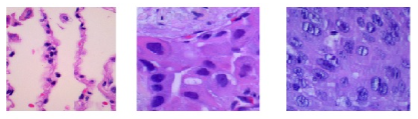
\includegraphics[width=8cm, height=4cm]{./figures/histo_img.png}}
\caption{Histopathological Images}
\label{histo_img}
\end{figure}

Histopathological with ML
Histopathological with DL,
Histopathological with Segmentation + DL

The authors in \cite{yu} have combined conventional thresholding and image processing techniques with machine learning methods, such as random forest classifiers, SVM or Naïve Bayes classifiers, achieving an Area Under the Curve (AUC) of ~0.85 in distinguishing normal from tumor slides, and ~0.75 in distinguishing LUAD from LUSC slides. In our work, we demonstrate how the field can greatly benefit from deep-learning using CNNs, which can automatically learn features from the image that may not be obvious to suspect and include during conventional image processing methods.

A whole slide histopathological image classification pipeline into five diagnostic categories of breast cancer using deep learning methods has been proposed in \cite{baris}. The pipeline involves 4 stages of localization procedure to identify the most diagnostically relevant sections of the WSI. This produces small and relevant patches for the classification. However, the extracted patches are directly classified, without any further reduction of potentially irrelevant parts of the image. In this paper, we propose to go one step further and extract only nuclear regions for classification.

In \cite{abdolhoseini}, the authors have addressed the problem in splitting heavily clustered nuclei due to its intensity variation caused by noise and uneven absorption of stains. A  multilevel thresholding method is applied followed by a watershed algorithm to separate clustered nuclei. Finally, a model-based merging step is applied to eliminate over-segmentation and a model-based correction step is used to improve segmentation results and eliminate small objects. In our paper, in addition to implementing a threshold-based segmentation, we have also trained a neueal network to perform automatic segmentation of nuclear regions.

A novel method for unsupervised segmentation of cell nuclei in stained histology tissue is presented in \cite{phoulady}. Following an initial preprocessing step involving color deconvolution and image reconstruction, the segmentation step consists of multilevel thresholding and a series of morphological operations. The only parameter required for the method is the minimum region size, which is set according to the resolution of the image.

The automated classification of adenocarcinoma and squamous cell carcinoma proposed in \cite{simon}, consists of a two-part approach. Firstly, they have implemented a deep learning framework to classify the input patches as adenocarcinoma, squamous cell carcinoma and non-diagnostic. Next, they extract a collection of statistical and morphological measurements from the labeled whole-slide image (WSI) and use a random forest regression model to classify each WSI as lung adenocarcinoma or lung squamous cell carcinoma.


A Deep Convolutional Neural Networks (DCNN) based feature learning was presented in \cite{xu2016deep} which automatically classify EP(Epithelial) and ST(Stromal) regions from digitized tumor tissue microarrays. An analysis pipeline which empowers the  spatial organization of cells and determines their roles in tumor progression and metastasis have been developed in \cite{wang2019convpath} using convpath. The pipeline consist of nuceli  segmentation and performs following cell type classification such as tumor cells, stromal cells and lymphocytes using the CNN. Automated classification scheme for microscopic images to classify three types of lung cancer such as Adenocarcinoma, Squamous cell carcinoma and  Small cell carcinoma was presented in \cite{teramoto2017automated}  using a deep convolution neural network. A deep neural network algorithm 





They have proposed an automatic end-to-end deep neural network algorithm for segmentation of individual nuclei. A nucleus-boundary model is introduced to predict nuclei and their boundaries simultaneously using a fully convolutional neural network \cite{cui2019deep}. 

nuceli segmentation:


This paper addresses the task of nuclei segmentation
in high-resolution histopathological images. We propose an automatic end-to-end deep neural network algorithm for segmentation of individual nuclei. A nucleus-boundary model is introduced
to predict nuclei and their boundaries simultaneously using a
fully convolutional neural network. Given a color normalized
image, the model directly outputs an estimated nuclei map and a
boundary map. A simple, fast and parameter-free post-processing
procedure is performed on the estimated nuclei map to produce
the final segmented nuclei. An overlapped patch extraction and
assembling method is also designed for seamless prediction of
nuclei in large whole-slide images. We also show the effectiveness
of data augmentation methods for nuclei segmentation task. Our
experiments showed our method outperforms prior state-of-the art methods. Moreover, it is efficient that one 1000X1000 image
can be segmented in less than 5 seconds. This makes it possible
to precisely segment the whole-slide image in acceptable time.

%In this study, the have trained a deep learning convolutional neural network (CNN) model (inception v3) on histopathology images obtained from The Cancer Genome Atlas (TCGA) to accurately classify whole-slide pathology images into adenocarcinoma (ADC), squamous cell carcinoma (SCC) or benign tumor cells \cite{coudray2018classification}. In this study, they have developed an automated classification scheme for lung cancers presented in microscopic images using a deep convolutional neural network (DCNN), which is a major deep learning technique\cite{teramoto2017automated}.

This study presents a comparative study of twelve nuclei segmentation methods for cytology pleural effusion images. Each method involves three main steps: preprocessing, segmentation, and postprocessing. preprocessing and segmentation stages help enhancing the image quality and extracting the nuclei regions from the rest of the image, respectively. postprocessing stage helps in refining the segmented nuclei and removing false findings. segmentation methods are quantitatively evaluated for 35 cytology images of pleural effusion by computing five performance metrics. Evaluation results show that the segmentation performances of the Otsu, k-means, mean shift, Chan–Vese, and graph cut methods are 94, 94, 95, 94, and 93\%, respectively, with high abnormal nuclei detection rates \cite{win2018comparative}.


In this study, to solve the
segmentation of nuclei and overlapping regions, we introduce a nuclei segmentation
method based on two-stage learning framework consisting of two connected Stacked
U-Nets (SUNets) \cite{kong2020nuclear}.



%Histopathological images contains nucleus and other components. The nucleus mutate and varies in size and structure if it found to be a malignant cell. The segmentation and analysis  of nuclei from tissue images is essential  because the cancer cells are heterogeneous shape and size features and immune cells of various shapes and sizes. Manual analysis is time consuming due to the hetrogeneous nature of the cell and subject to inter and intra observer variability.Since the histopathological image of the lungs contains different components classification of the whole slide histopathological image may reduce the accuracy of the system. 


%Classification with the help of the machine learning technique requires manual feature engineering which also reduces the classification accuracy. Hence we proposed to develop an automated system using a deep learning technique to classify the histopathological lung tissue as benign or malignant after segmenting the nuclei based on the color information. The proposed an system that segments the  nucleus using 
image processing technique such as thresholding and contour based. The segmented nucleus present in the histopathological images are classified as  benign and malignant. The histopathological images are made up of  different structures such as the nucleus, chromosomes, cytoplasm, lymphocytes etc.

\textbf{
The methods proposed and work detailed in this paper have the following key highlights
\begin{itemize}
    \item An Xception-style UNet with skip connections is experimented and proposed to segment nuclei from a Whole Slide Histopathological Image (WSHI) patch. The network achieves a mean-IoU of 0.9427 on the test data.
    \item An algorithmic method of generating masks as ground-truth for training and testing the UNet network is proposed. The method is based on contour detection and color-based filtering techniques.
    \item A Deep Convolutional Neural Network (DCNN) is proposed to perform binary and multi-class classification of lung tumors using complete WSHI patches as well as segmented nuclei information obtained through the proposed deep learning segmentation network.
\end{itemize}
}

\section{Overview of Proposed System}

In this paper, we propose a Deep Convolutional Neural Network (DCNN) that performs \emph{two forms} of classification of the histopathological lung images --- binary and multi-class. While binary classification identifies an input  image as either benign or malignant, multi-class classification will assign one of three classes to an input image --- ADC, SCC and Benign. 

The nuclei of benign and cancerous lung tissues are known to posses visually distinguishable characteristics. Furthermore, each sub-type of lung cancer affects these characteristics differently. Limiting the information available in the input images to only these relevant regions that impact classification, can improve the classifier's performance. A DCNN classifier extracts features from the information available to it. When only nuclear regions are available, the effort of the DCNN in learning to suppress the weights of less relevant features stemming from other regions of the image is greatly reduced. Moreover, retaining only the nuclear regions from a WSHI patch gives rise to images that mask the non-nuclear regions with sharp gradients at the nucleus boundaries. As a result of such highly pronounced boundaries, shape-based features will be learnt much more robustly and rapidly.

Hence, we propose to improve the classification accuracy of the DCNN by performing semantic segmentation to retain only the nuclear regions of the input WSHI patches. We present an Xception-style UNet for semantic segmentation, along with \emph{two different approaches} to prepare the ground-truth for training this network. Further, we study and present the difference in performance of the classifier when it is trained with input images that contain only the segmented nuclear regions from when the entire WSHI patches are employed.  

\begin{figure}[htbp]
\centerline{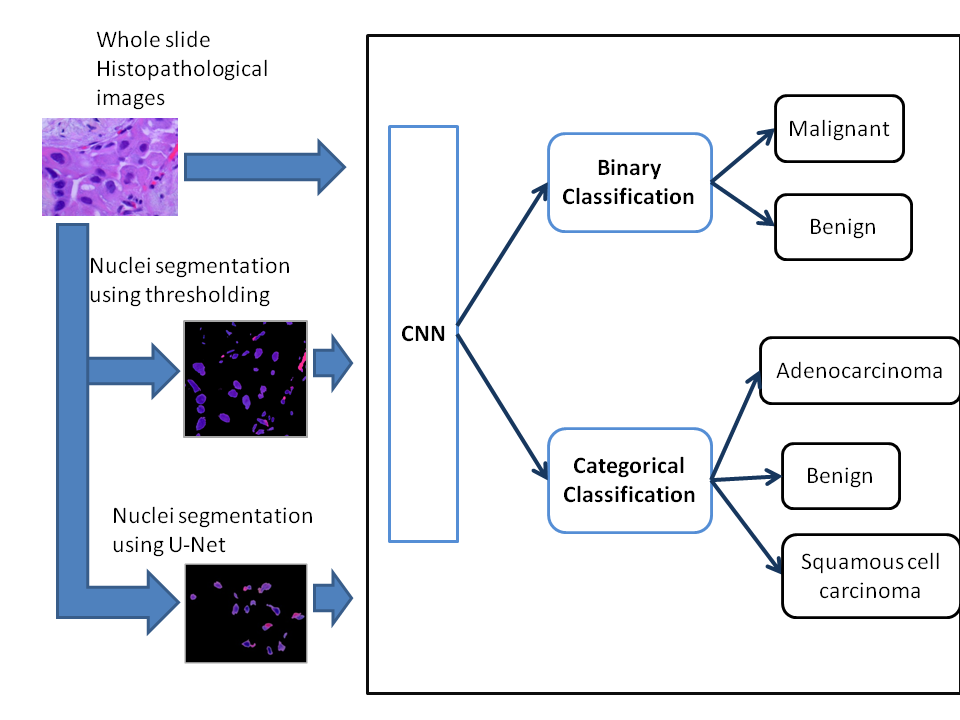
\includegraphics[width=9cm, height=7cm]{./figures/proposed_system.png}}
\caption{Proposed system}
\label{proposed sys}
\end{figure}

\subsection{Preliminiary Preprocessing}
\label{sect_datapreprocess}
Our proposed methodology involves training a DCNN to perform classification. To avoid over fitting, to adopt a diversity-based sampling strategy and to cater to the large input requirement of the deep learning network, data augmentation is necessary. Random affine transformations such as rotation, scaling and shearing are applied to augment the input data. The input images are resized to 128x128, 3-channel images using bi-linear interpolation. The images are then linearly-normalized to envelope the pixel values between 0 and 1. This is known to improve the rate of convergence and enhance the network's ability to standardize to diverse inputs.

\subsection{Input Image Preparation}

After the preliminary stage of preprocessing, two different pipelines are adopted --- the first, feeds the preprocessed WSHI patches to the classifier directly and the second, extracts only the nuclear regions of the input images and passes them to the classifier.

The second pipeline is of particular interest, which involves performing an automated semantic segmentation of the preprocessed WSHI patches to retain only the nuclear information from the image. This is achieved with the help of a segmentation network which takes an input WSHI patch and produces a binary mask image. A binary mask is an image with the same dimensions as the input image, but the pixel values are replaced with a numeric class label to classify the corresponding pixels in the input image into one of two semantic class --- namely, nuclear and non-nuclear regions. To this effect, the mask encodes nuclear regions with a class label of 1 and 0 otherwise. 

A \emph{bitwise-AND} operation is performed between the input RGB image of the WSHI patch and the generated mask. The result of this operation is an image containing only the information corresponding to the nuclear regions of the input WSHI patch as encoded in the mask. This operation is depicted in the Figure \ref{result}. In the second pipeline, the image so obtained is passed to the DCNN classifier. The specific details about the segmentation network and the methods adopted to prepare the ground truth for training the network are included in a subsequent section (section-\ref{sec4_segmentation}).

\subsection{Binary and Multi-Class Classification}

The input WSHI patch images, after being processed through one of the pipelines, is relayed to a DCNN classifier. Two variants of the classifier are proposed --- one for binary classification and the other for multi-class classification. The binary classifier labels the input WSHI patch as either benign or malignant, and the multi-class variant goes one step further and assigns one of three classes to an input image --- ADC, SCC and Benign, where ADC and SCC are sub-classes of the malignant type.

The two variants of the classifier are kept consistent across all the pipelines to evaluate and contrast between the quality of classification achieved through each of the different input preparation methods and segmentation approaches adopted. The classifier network architecture and its variants as well as an analysis of the results obtained through each method are detailed in separate subsequent sections (section-\ref{sec5_classifier} and section-\ref{sec6_results}).

\section{Semantic Segmentation to Extract Nuclear Regions}
\label{sec4_segmentation}
The second pipeline proposed for classification involves extracting nuclear regions of the input WSHI patches through semantic segmentation. We propose an Xception-style UNet architecture to perform this binary segmentation. The remainder of this section provides some background on the rationale behind the methods adopted to prepare the ground-truth for semantic segmentation, the preparation procedure and details of the network architecture used in this work.

\subsection{Ground Truth Preparation}

During a histopathological examination, the obtained tissue samples are prepared on microscope slides for visual examination, typically using methods such as chemical fixation and frozen section processing. Such slides are stained using coloring pigments to reveal and distinguish cellular components. Hematoxylin and Eosin (H\&E) is the most commonly used stain combination. Hematoxylin reacts like a basic dye with specific cell components --- namely the cell nucleus, ribosomes and the endoplasmic reticulum. The basic reaction stains these cell components with a purplish-blue color. On the other hand, Eosin is an acidic dye that affixes the cytoplasm, cell walls and extracellular connective matrix of the tissue with a dull reddish-pink stain. These slides can then be examined under a microscope by pathologists or micrographed to produce WSHIs. 

The WSHI patch images used in this study are stained using H\&E. On account of staining, the nuclear regions (as well as some other cellular components) in the histopathological images have significantly different visual properties than the remainder. The visual properties of any image pixel can be broadly categorized into two --- \emph{chroma} and \emph{luma}. While \emph{chroma} represents the color of a pixel, \emph{luma} encodes the intensity level of that color in the pixel. Based on this categorization, two different approaches to extracting the nuclear regions from the WSHI patches can be conceived --- one based on intensity variations and the other, rooted at color distinctions. These approaches are pursued to prepare the ground-truth masks required to train the segmentation network. 

It is worth noting, that while Hematoxylin stains all the nuclear regions of the tissue, it stains a few other cellular components as well --- namely, the ribosomes and the endoplasmic reticulum.  Hence, a segmentation procedure that obtains the nuclear regions based on the variations introduced by staining, will inevitably include some portions of the non-nuclear regions as well. These portions are regarded as noise. However, the intention behind the approach proposed in the second pipeline is to limit the image regions available to the classifier to contain only the most relevant information. Hence, as long as none of the nuclear regions of the image are lost to segmentation, allowing some non-nuclear regions of the image to persist in the segmented input is not detrimental. It will not degrade the classification performance any more than passing the entire WSHI patch, as is the case in the first pipeline. In the remainder of this paper, the mention of nuclear regions in the context of segmentation, implicitly includes the noise that may accompany it. 

\subsubsection{Based on Intensity Variation}

This approach to segmenting the nuclear information from input WSHI patches leverages the intensity variations in the visual structure of the WSHI patches due to staining. The nature of staining leaves the pixels of the nuclear regions with a darker shade and hence a higher intensity value, relative to the remainder of the image.

The input patch images are first converted to grayscale to retain only the intensity information of pixels \cite{hui_liu} and discard the color details. Otsu's method \cite{otsu}, a global thresholding method that determines an optimal threshold to segregate the pixels in a given image into two classes with minimum intra-class variance and maximum inter-class differentiation, is then applied to obtain an image-global intensity threshold value. In effect, these two classes of pixels correspond to the nuclear and non-nuclear regions of the WSHI patch, with the higher intensity class representing the former.

The pixels with intensity values lower than the obtained threshold are folded down to a value of 0 while the remainder are set to 1, thereby generating a binary image. Semantically, this image retains an extract of the WSHI patch that contains only the nuclear regions of the image, as identified by the thresholding technique, by encoding those pixels with an intensity value of 1. The binary image is then extrapolated into a three-channel image by duplicating the only channel present. This serves as a binary mask that can be used to extract nuclear information from the corresponding WSHI patch by performing a \emph{bitwise-AND} operation between the two.

\begin{comment}
A bitwise 'and' operation is performed between the input RGB image of the WSHI patch and the generated mask. The result of this operation is an image containing only the information corresponding to the nuclear regions of the input WSHI patch as identified by the thresholding technique. This operation is depicted in the Figure \ref{result}. This final image serves as a mask. 
\end{comment}

The WSHI patch image and the corresponding binary mask serve as input and annotation respectively, to train the segmentation network. 

\subsubsection{Based on Color Distinction}

Staining histopathological slides with H&E, attributes a purplish-blue color to the nuclear regions of the image. In this approach, nuclear information is extracted from input WSHI patches by exploiting this color distinction as well as the intensity variations that arise in the visual structure of the WSHI patches on account of staining.

The input WSHI patch is first partitioned into several sub-regions. A sub-region here, refers to the set of pixels enclosed within each boundary representing a subset the image area. This is done using Suzuki's contour detection algorithm \cite{suzuki} and it uses the variation in intensity of pixels to achieve this. These variations are more pronounced at the boundary between nuclear and non-nuclear regions of the image and as a result, transitioning from a nuclear component of the image to an adjacent non-nuclear region is characterized by a sharp change in the pixel intensity values. These abrupt variations are detected by the contour detection algorithm to find closed loop boundaries within the image, that separate adjacent nuclear and non-nuclear components. The boundaries so obtained are stored as a vector of continuous pixels forming a closed loop and can be applied on the WSHI patch to obtain sub-regions. In effect, the image is partitioned into a large number of sub-regions, some pertaining to nuclear regions and the others representing non-nuclear components in the patch. 

The WSHI patch with the obtained sub-regions is a RGB image. RGB images encode \emph{chroma} and \emph{luma} information in an inter-mixed manner. The Hue-Saturation-Value (HSV) image format on the flip side, separates the two, with the hue component encoding all the \emph{chroma} information and the Saturation and Value components containing the \emph{luma} information about color saturation and brightness, respectively. 

In order to use only the color information, the WSHI patch is now converted to the HSV format. For each sub-region in the patch image, the average hue component value is computed. A suitable range of average hue values that can describe the nuclear sub-regions is arrived at, using expert guidance. Finally, the sub-regions having average hue values within this range are retained in the WSHI patch image, discarding the rest. These sub-regions are then used to produce a corresponding binary mask image with nuclear regions encoded with a pixel value of 1 and the non-nuclear regions i.e the regions discarded from the patch image, marked as 0. The resulting mask image, therefore, serves as an extract of nuclear information.

When determining the hue value range, a trade-off must be made between two options that arise from the inherent approximation associated with the method used to find the sub-regions. On one hand, the segmented image can be restricted to disallow any component apart from the nucleus at the expense of losing some nuclear information. On the other hand, it can be ensured that the segmented image has all the nuclear information at the cost of allowing some portions of other components. The latter is chosen, since feeding some extra information to the classifier DCNN, while guaranteeing the presence of all nuclear information, is a more justified approach than compromising important nuclear information.

As in the previous approach, the WSHI patch image and the corresponding binary mask so obtained, serve as input and annotation respectively, to train the segmentation network. 

\subsection{Segmentation Network Architecture}

The UNet \cite{jonathan} is a Convolutional Neural Network architecture, proven for segmentation of medical images. The segmentation of nuclei information from the WSHI requires just two semantic classes --- nuclear and non-nuclear regions. An initial experiment with a simple UNet architecture showed accuracy saturation and high training loss, suggestive of the degradation problem \cite{kaiming}. Hence, we propose an Xception-style \cite{chollet} UNet architecture, to employ residual blocks that can reduce degradation in deep networks and easily adapt to learning simplex as well as complex correlations between the layers of the network \cite{veit}. Concurrent with the standard UNet structure, the proposed architecture consists of a contractive downsampling path followed by an expansive upsampling path. The input images are first resized to $512\times512$ with 3 channels and passed through an entry block. This block comprises of a convolution layer with a standard kernel size of $3\times3$, a batch-normalization layer and a Rectified Linear Unit (ReLU) activation layer. The block produces an output with 32 channels.
 
The contracting path is composed of three blocks with progressively increasing filter sizes of 64, 128 and 256. The intention is to learn about the existence of distinctive finer features as the image percolates deeper into the network. Separable Convolution layers are used, which perform depth-wise spatial convolutions followed by point-wise convolutions that mix the output channels. The approach is adopted with the supporting hypothesis on Xception networks that cross-channel correlations and spatial correlations can be treated as being entirely disengaged. In each block, two sets of convolution layers, each preceded by a ReLU activation layer and followed by a batch normalization layer is applied. This sequence is followed by a max-pooling layer and an addition-based skip connection from the input to the current block. The placement and ordering of the layers within each block determines the nature of activation. As discussed in \cite{kaiming}, pre-activation and post-activation produce significantly distinct network performances in the presence of element-wise addition. Element-wise addition is introduced by the use of residual connections. Specifically, pre-activation produces better regularization by reducing overfitting and eases optimization due to a more direct weight propagation between subsequent blocks, when the relationship between them is more closer to an identity mapping rather than a complex function. The ReLU-only pre-activation and the full pre-activation approaches discussed in \cite{kaiming} were experimented with, and the former approach was found to produce better results. Concretely, the sequence shown in sequence-(\ref{unet-contract-sequence}) is adopted within each block of the downsampling strata.

\begin{equation}
\label{unet-contract-sequence}
SkipConnectionStartPoint  \rightarrow ReLU \rightarrow Convolution \rightarrow BatchNormalization \rightarrow ReLU \rightarrow Convolution \rightarrow BatchNormalization \rightarrow MaxPooling \rightarrow SkipConnectionEndPoint 
\end{equation}

The latter half of the network is an expanding path that uses transposed convolutions \cite{dumoulin} to upsample the low resolution image at the end of the contracting path progressively, back to its original resolution. A single step of transposed convolution is achieved by performing convolutions on the image obtained by sufficiently zero-padding around each pixel of the low resolution image. In effect, the subsequent series of downsampling and upsampling operations, recovers the spatial information lost during the contraction phase and further, localizes the identified features to their corresponding positions on the higher resolution image produced at each step of the expansion path. Ultimately, pixel-wise classification into semantic classes is perfomed on these localized features once the original resolution is reached. To further enhance the precision of mapping between features and their respective locations on the upsampled image and avoid losing fine-grained information, skip connections are used to forward and concatenate features from corresponding stages of the contraction path with the upsampled image obtained at the same stage of expansion path. In particular, the use of skip connections is known to help with feature reuse and is the most notable purpose of employing them in the segmentation network. However, shorter skip connections are also known to alleviate the vanishing gradient problem \cite{hochreiter, drozdzal}.

The transpose convolution blocks used in the expansion path have a symmetric structure with respect to the contracting path. It comprised of three blocks with progressively decreasing filter sizes of 256, 128 and 64.
Following the symmetric structure, each block is constructed with two sets of transpose convolution layers, each followed by a ReLU activation layer and followed by a batch normalization layer. This is followed by an upsampling layer and an addition-based skip connection to forward features from the current block's input to output. Once again, the sequence of layers in each block follows the ReLU-only pre-activation strategy. Notably, the upsampling layer is different from a convolution transpose layer in that the former simply doubles the dimensions of its input while the latter performs an inverse convolution operation and learns the kernel during the training phase. In particular, each block of the upsampling strate follows the sequence depicted in sequence-(\ref{unet-expand-sequence})

\begin{equation}
\label{unet-expand-sequence}
SkipConnectionStartPoint  \rightarrow ReLU \rightarrow Convolution \rightarrow BatchNormalization \rightarrow ReLU \rightarrow Convolution \rightarrow BatchNormalization \rightarrow UpSampling \rightarrow SkipConnectionEndPoint 
\end{equation}

Two variants of this network are trained using complete WSHI patches and their corresponding annotation masks obtained using the two ground truth preparation approaches. When the second pipeline is adopted for classification, the input WSHI patches are passed through each of these variants to obtain segmentation masks. The \emph{bitwise-AND} operation is performed between the masks and the  input patch images to produce an image containing the segmented extract of only the nuclear regions. Finally, this extract image is passed to the DCNN classifier. The quality of segmentation obtained from each variant of the network as well as the final classification performance resulting from each of the ground truth preparation approaches is compared and analyzed in a subsequent section (section-\ref{sec6_results}).

\section{Classification of Lung Tumor Cells}
\label{sec5_classifier}

\subsubsection{Complete WSHI Patches}
In this approach, the input images obtained after data augmentation are directly fed to DCNN for classification. Consequently, the features extracted by the network for classification are not limited to the nuclear regions, but span throughout the input WSHI patch. This is the most commonly adopted strategy in histopathological image classifiers. We have included this method in our work to establish a baseline performance measure of the proposed DCNN classifier. This baseline is used to study and discriminate the impact of segmenting out nuclear features from the WSHI patches on the accuracy of classification. 

\subsubsection{Intensity Based Thresholding to Segment the Nuclear Information}

This approach to segmenting the nuclear information from WSHI patches utilized the intensity variations of n  

The WSHI patch images used in this study are stained using H&E. Hence the nuclei and Since different components of the histopathological images are stained differently, we propose  to  segment the nucleui from the WSHI based on the color variations. Due to the nature of staining, the nuclei is always of a brighter shade in the grayscale images. This characteristic is exploited to segment the nuclei from the WSHI. 
 
Image pixels are charecterized by color and intensity
 
 images are converted into a gray-scale image. Otsu's method, a global thresholding method that determines an optimal threshold for the given imagethat minimizes the intra-class variance between the nucleus and non-nucleus sections of the image, is used to obtain a threshold. The pixel values lower than the obtained threshold are set to 0, while the others are set to 1. The output image contains segmented nucleus in the binary form along with some noise, stemming from other stained parts of the cells.  The output is converted into a 3-channel image by duplicating the only channel present and a bit-wise 'and' operation is performed with the RGB input image. This extracts and retains only the information corresponding to the regions identified as nuclear information by the thresholding technique, from the WSHI. This operation is depicted in the Figure \ref{result} 

\textbf{
We propose a CNN model comprising of six convolution blocks. Each block contains a convolution layer, an activation layer, a batch-normalization layer and a max-pooling layer. Each block consists of a convolution followed by activation layer, a batch normalization layer and a pooling layer. Dropout layers are added at the end of alternate convolution blocks to prevent over-fitting. The convolution blocks extract distinctive features from the input images. The initial layers extract high-level features. As the images percolate through the deeper layers of the network, the channel-size is increased progressively from 32 to 128 to extract more subtle features that can help in inter-class differentiation. The feature representation vectors obtained from the convolution layers are flattened using the flatten layer and fed into the classification layer. The classification layer consists of two dense stages. The first stage includes a dense layer followed by an activation layer and a dropout layer. The second stage, which is the output layer, includes a dense layer followed by an activation layer. The activation layer consist of a single neuron for binary classification and three neurons for multi-class classification.
}

\textbf{
In the proposed CNN model, we have used 2D separable convolution layers with a filter size of 32, kernel size of 3x3 and a stride length of 1. It performs channel-wise spatial convolution followed by a point- wise convolution while mixing the output channels. Rectified Linear Unit (ReLU) function is used to activate the hidden layers while the Softmax function is used for the dense layers. The model is fed with 32 input images per batch and trained using the Nesterov-accelerated Adaptive Moment Estimation (NAdam) optimizer with a learning rate of 0.001. The dropout layers have a dropout rate of 0.50 in the dense layer and 0.25 in the convolution layers. We have conducted experiments to perform both binary as well as multi-class classification using the proposed DCNN model.
}

\subsection{Classification using WSHI}

In our proposed work, we classify the WSHI using the proposed DCNN. The WSHI images are pre-processed as described in section \ref{sect_datapreprocess} and fed to the DCNN. Two different classifications are performed - binary classification into malignant and benign, multi-class classification into ADC, SCC and benign.  

\begin{comment}
The deep learning model needs to learn features from the images, so it is necessary to have large amount of images. We have applied data augmentation technique to generate more images by applying different transformation technique such as rotation, flipping and scaling on the input images. We have  generated images by performing  the rotation range of 20 degrees, zoom range as 0.05, height shift range and width shift range as 0.1, horizontal flip, vertical flip and random flip.
\end{comment}

\subsection{Classification using nucleus segmented by thresholding}

 The histopathological images are stained using Hematoxylin and Eosin (H\&E) which provides the pathologist a detailed view of the tissue. Hematoxylin reacts with specific cell components like a basic dye to produce a purplish blue colour. It stains the cell nucleus, ribosomes and endoplasmic reticulum. Eosin is an acidic dye that is typically reddish or pink. It stains the cytoplasm, cell walls, and extracellular fibres of the tissue cells. Since different components of the histopathological images care stained differently, we propose  to  segment the nucleui from the WSHI based on the color variations. Due to the nature of staining, the nuclei is always of a brighter shade in the grayscale images. This characteristic is exploited to segment the nuclei from the WSHI. 
 
 The input histopathological RGB images are converted into a gray-scale image. Otsu's method, a global thresholding method that determines an optimal threshold for the given that minimizes the intra-class variance between the nucleus and non-nucleus sections of the image, is used to obtain a threshold. The pixel values lower than the obtained threshold are set to 0, while the others are set to 1. The output image contains segmented nucleus in the binary form along with some noise, stemming from other stained parts of the cells.  The output is converted into a 3-channel image by duplicating the only channel present and a bit-wise 'and' operation is performed with the RGB input image. This extracts and retains only the information corresponding to the regions identified as nuclear information by the thresholding technique, from the WSHI. This operation is depicted in the Figure \ref{result} 

\begin{figure}[htbp]
\centerline{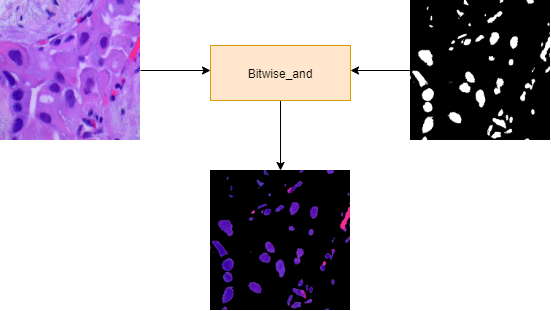
\includegraphics[width=8cm, height=5cm]{./figures/result.png}}
\caption{Bitwise And Operation}
\label{result}
\end{figure}

The segmented nuclei are obtained by performing the threshold technique is depicted in the Figure \ref{threseg} which is used for further classification by a CNN model.
\begin{figure}[htbp]
\centerline{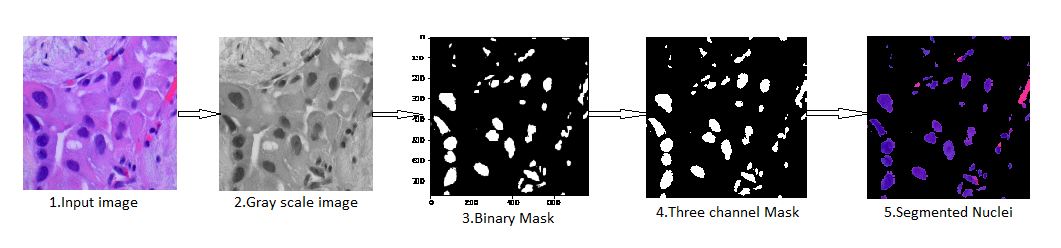
\includegraphics[width=10cm, height=4cm]{./figures/threseg.png}}
\caption{Threshold based Segmentation}
\label{threseg}
\end{figure}

\begin{comment}


\subsubsection{Color Based Segmentation of Nucleus}.

The input histopathological images are obtained by stained using H&E stains. As a result, the nuclei are purple colored. The classification into malignant and benign can be done based on the structure analysis of the nucleus. In order to segment the nuclei, the RGB input image is converted into grayscale. Contours are found on the grayscale histopathological image, segmenting it into several sections based on pixel intensity variation boundaries. The average hue value was computed for the pixels present within each of these contours. Contours having an average hue value in the range 154-170 are purple and these contours alone were extracted out. The segmented nuclei obtained, are used for further classification using a CNN model.




\section {Classification}
The segmented nucleus, obtained from the aforementioned methods, are classified using a Deep Convolution Neural Network (CNN) model. The performance of the two different methods have been analyzed in the following sections.

Our proposed CNN model consists of 6 convolution layers and 2 dense layers. Each convolution layer is followed by an activation layer, batch normalization layer and a max-pooling layer. The architectures extracts generic features in the initial layers and image-specific features in the final layers. The features obtained are flattened using a flatten layer and fed to the classification layer. The classification layer consists of two dense layers. The first dense layer is followed by an activation function and dropout layer. The final dense layer only includes an activation function. The output layer, has only one node in case of binary classification into benign and malignant and 3 nodes to perform multi-class classification into adenocarcinoma, squamous cell carcinoma and benign. The ReLU function is used for activation of the dense layers, whereas the Softmax function is used for the output layer. A dropout rate of 0.25 is used in the dense layer.


The proposed binary classification system classifies the lung cancer types into malignant and benign from color based segmented nuclei and categorical classification system classifies the lung cancer types into adenocarcinoma, squamous cell carcinoma and benign using color based segmented nuclei. 
\end{comment}

\subsection{Classification using nucleus segmented by UNet model}

In this method, we propose a deep learning UNet model to segment the nuclei from the WSHI. The segmented nucleus is further classified using the proposed DCNN.

\subsubsection{Data Preparation}
\textbf{
We propose an automated ground truth preparation of nucleus mask to train the UNet model to segment the nuclei from WSHI on the fly. Each histopathological image contains one or more nuclei in addition to other cell-level components. The images are obtained after being dyed for microscopic analysis using H&E. The  ground preparation process involves obtaining an input WSHI and creating a mask that segments and retains only those pixels of the input image that belong to a nucleus. This is achieved using a contour detection method and color based filtering under expert guidance.}

\textbf{
The input WSHI is first converted into a binary image to amplify the inter-component boundary separation. These boundaries, separating different components of the image, are used to divide the input image into several sub-regions using a contour detection algorithm. As a result of staining, the nucleus components of the image have a clearly distinguishable boundary are easily identified as separate sub-regions. A large number of sub-regions are identified, but only some of these regions correspond to nuclear information. To recover the color information, the sub-region boundaries obtained on the binary image are translated back to the original WSHI. 
}

\textbf{
The WSHI with the obtained sub-regions is a RGB image. RGB images contain inter-mixed chroma (color) and luma (intensity) information. However, due to staining, the nuclear sub-regions of the image can be identified by using only the chroma information. Hence, the WSHI is converted to the Hue-Saturation-Value (HSV) image format. The HSV image contains chroma information in the hue component and luma information about the color saturation level and brightness in the saturation and value components, respectively.
}

\textbf{
For each sub-region in the WSHI, the average hue component value is computed. A suitable range of average hue values which can describe the nuclear sub-regions is arrived upon using expert guidance. When choosing the range limits, a trade-off has to be made between two options that arise from the inherent approximation associated with the sub-region finding method. On one hand, the segmented image can be restricted to disallow any component apart from the nucleus at the expense of losing some nuclear information. On the other hand, the segmented image can be ensured to have all the nuclear information at the cost of allowing some portions of other components. The latter is chosen since feeding some extra information while guaranteeing presence of all nuclear information to the classifier DCNN is a justified choice than losing important nuclear information. Once the range is decided, only those sub-regions falling within this range are retained in the WSHI image. The corresponding sub-regions are then used to produce a binary mask with nuclear regions marked as 1 and non-nuclear regions marked as 0. The resulting mask image contains all regions containing nuclear information with possibly some additional information. 
}

\textbf{
This method was adopted to prepare a ground-truth of 6000 images and corresponding nuclei masks. These images were split in 80:20 ratio to train and test the UNet semantic segmentation model proposed in section \ref{sect_unet_arch}. 
}

\begin{comment}
< Black background images *mask >
\end{comment}

\subsubsection{U-Net architecture}
\label{sect_unet_arch}

\textbf{
The U-Net \cite{jonathan} is a Convolutional Neural Network architecture, proven for segmentation of medical images. The segmentation of nuclei information from the WSHI requires just two semantic classes - nuclei and non-nuclei. An initial experiment with a simple UNet architecture showed accuracy saturation and high training loss, suggestive of the degradation problem. Hence, we propose a Xception-Style \cite{chollet} UNet architecture, to employ residual blocks that can reduce degradation in deep networks and easily adapt to learning simplex as well as complex correlations between the layers of the network \cite{veit}. Concurrent with the standard UNet structure, the proposed architecture consists of a contractive downsampling path followed by an expansive upsampling path. The input images are first resized to $512\times512$ with 3 channels and passed through an entry block comprising of a convolution layer with a standard kernel size of $3\times3$ and a batch-normalization layer followed by Rectified Linear Unit (ReLU) activation. The layer produces an output with 32 channels.
}

\textbf{
The contracting path is composed of three blocks with progressively increasing filter sizes of 64, 128 and 256. The intention is to learn about the existence of distinctive finer features as the image percolates deeper into the network. Separable Convolution layers are used, which perform depth-wise spatial convolutions followed by point-wise convolutions that mix the output channels. The approach is adopted with the supporting hypothesis of Xception networks that cross-channel correlations and spatial correlations can be treated entirely disengaged. In each block, two sets of convolution, ReLU activation and batch normalization layers are applied. This is followed by a max-pooling layer and an addition skip connection from the input to the current block. The placement of the layers within each block determines the nature of activation. As discussed in \cite{kaiming}, pre-activation and post-activation produce significantly distinct in network performances in the presence of element-wise addition. Element-wise addition is introduced by the use of residual connections. Specifically, pre-activation produces better regularization by reducing overfitting and eases optimization due to a more direct weight propagation between subsequent blocks when the relationship is closer to identity mapping than a complex function. The ReLU-only pre-activation and full pre-activation approaches discussed in \cite{kaiming} were experimented with and the former approach was found to produce better results. Concretely, the sequence shown in sequence \ref{unet-contract-sequence} is adopted within each block of the downsampling strata.
}

\begin{equation}
\label{unet-contract-sequence}
ReLU \rightarrow Convolution \rightarrow BatchNormalization \rightarrow ReLU-Convolution \rightarrow BatchNormalization \rightarrow MaxPooling \rightarrow SkipConnection 
\end{equation}

\begin{comment}
Added detailed content for UNet contraction path
Included 5 mroe citations
Will add for UNet expansion path
\end{comment}

The decoder part uses transposed convolution to permit localization using fully connected layers. The decoder uses skip connections to concatenate the feature map in the same stage. Thus the segmentation network is capable of utilizing multi-scale image features to learn the nuclei mask for each histopathological images. The segmented nucleus are compared with the input mask with the help of Intersection of union. The nuclei segmented using the UNet model are further classified using the proposed CNN models.

 \section{Experiments and Results}
\label{sec6_results}
The experiment consisted of two major forms of classification of lung cancer types --- from the WSHI of lung tissues and from the nuclear regions segmented out of the lung tissue WSHIs. Both forms of classification were performed using deep learning techniques. Two methods were experimented with, to perform the segmentation of the nuclear regions from the WSHI --- a image-wise global thresholding based method and a deep-learning approach using an Xception-style UNet model. The results of these experiments are analyzed using different metrics such as accuracy, F1 score, sensitivity and specificity for each classification approach and presented in sections \ref{exp_WSHI}, \ref{exp_thresh} and \ref{exp_unet}, to ascertain the performance of the proposed system.

\subsection{Dataset}
The data-set consisted of 15000 color images belonging to three classes with 5000 images each. All the images are 768x768 pixel size stored in the JPEG file format. The three classes are lung adenocarcinoma, squamous cell carcinoma and benign lung tissues \cite{conf-dataset}.  To avoid over fitting and to adopt diversity-based sampling strategy data augmentation and to cater to the large input requirement of the neural-network, data augmentation is necessary. Random affine transformations such as rotation, scaling and shearing methods are adopted.


\subsection{Classification using CNN from Whole slide Histopathological Images}
\label{exp_WSHI}

In this approach, the WSHIs images available from the data-set are used to train the neural network. The first form of classification performs a binary prediction of each input image into one of benign and malignant types. A total of 8000 images with 4000 images from each of the benign and malignant classes are used to train the network for 25 epochs at a learning rate of 0.01. The Nesterov-accelerate (NAdam) optimizer was used and the model reached a convergence loss of 0.0214 with an accuracy of 85.24\%. The network was evaluated using a test-set of 2000 images --- 1000 images from each class where it achieved a classification accuracy of 96.54\% on the training dataset and 95.70\% on the testing dataset. The confusion matrix for this classification is summarised in Table \ref{table1}.

\renewcommand{\arraystretch}{1.2}
\begin{table}[!htb]
\begin{center}
\begin{tabular}[scale=2.0]{|m|c|c|c|}
  \hline
  \multicolumn{2}{|c|}{\multirow{5}{*}{Types}}&\multicolumn{2}{c|}{\textbf{Predicted}}\\\cline{3-4}
  \multicolumn{2}{|c|}{} & & \\
  \multicolumn{2}{|c|}{} & \textbf{Benign} & \textbf{Malignant}\\
  \multicolumn{2}{|c|}{} & & \\\cline{1-4}
  & & & \\
  \multirow{3}{*}{\rotatebox[origin=c]{90}{\textbf{Actual}}}& \textbf{Benign} & 1000  &  0 \\
  & & & \\\cline{2-4}
  & & & \\
  &\textbf{Malignant} & 86  &  914 \\
  & & & \\\cline{1-4} 
\end{tabular}
\caption{Confusion matrix for Binary classification from whole slide histopathological images}
\label{table1}
\end{center}
\end{table}

It is evident from the confusion matrix that all the benign tissues have been classified with a 100\% accuracy  the malignant type have not been classified perfectly.


We have also performed multi-class classification of the input images into three classes - adenocarcinoma, squamous cell carcinoma and benign tumor. The results are summarized as a confusion matrix in table \ref{table2}. The network has been trained for 25 epochs and attained a loss error value 0.0341, The network achieved a 95.14\% training accuracy and 94.96\% testing accuracy. 

\renewcommand{\arraystretch}{1.2}
\begin{table}[!htb]
\begin{center}
\begin{tabular}[scale=2.0]{|m|c|c|c|c|}
  \hline
  \multicolumn{2}{|c|}{\multirow{4}{*}{Types}}&\multicolumn{3}{c|}{\textbf{Predicted}}\\\cline{3-5}
  \multicolumn{2}{|c|}{} & & &\\
  \multicolumn{2}{|c|}{} & \textbf{Benign} & \textbf{ADC} & \textbf{SCC}\\
  \multicolumn{2}{|c|}{} & & &\\\cline{1-5}
  & & & &\\
  \multirow{3}{*}{\rotatebox[origin=c]{90}{\textbf{Actual}}}& \textbf{Benign} & 992 & 8 & 0\\
  & & & &\\\cline{2-5}
  & & & &\\
  &\textbf{ADC} & 0 & 1000 & 0\\
  & & & &\\\cline{2-5} 
  & & & &\\
  &\textbf{SCC} & 143 & 0 & 857 \\
  & & & &\\\cline{1-5} 
\end{tabular}
\caption{Confusion matrix for Categorical classification from whole slide histopathological images}
\label{table2}
\end{center}
\end{table}


From the table \ref{table2} it has proved the model is good enough  to classify the malignant types - ADC and SCC. All the test images of ADC have been correctly classified. However, some of the SCC images have been mis-classified as ADC. Nonetheless, it has still been classified under a malignant category, which draws the attention of the medical experts to treat immediately. On the other hand, some of the benign images have been classified as ADC. This is because, the histopathological images contain many structures and the model learns features considering the entire image. This could be a cause for the reduced accuracy of the model. This can be overcome by classifying images considering only the nuclei in the image.




\subsection{Threshold Based Segmentation}
\label{exp_thresh}

The nuclei which have been segmented from the Whole Slide histopathological images based on the thresholding technique, have been further classified using the proposed CNN model. The dataset is split into training and testing sets in 80:20 ratio with equal number of images from each class, for both binary and multi-class classification. 

To perform binary classification into malignant and benign, the network was trained for 100 epochs at learning rate of 0.01 using the NAdam optimizer. With a final loss of 0.0478, the network achieved a training accuracy of 99.04\% and a testing accuracy of 98.45\%. The confusion matrix in table \ref{table3} represents the classification results.

\renewcommand{\arraystretch}{1.2}
\begin{table}[!htb]
\begin{center}
\begin{tabular}[scale=2.0]{|m|c|c|c|}
  \hline
  \multicolumn{2}{|c|}{\multirow{5}{*}{Types}}&\multicolumn{2}{c|}{\textbf{Predicted}}\\\cline{3-4}
  \multicolumn{2}{|c|}{} & & \\
  \multicolumn{2}{|c|}{} & \textbf{Benign} & \textbf{Malignant}\\
  \multicolumn{2}{|c|}{} & & \\\cline{1-4}
  & & & \\
  \multirow{3}{*}{\rotatebox[origin=c]{90}{\textbf{Actual}}}& \textbf{Benign} & 971  &  29 \\
  & & & \\\cline{2-4}
  & & & \\
  &\textbf{Malignant} & 2  &  998 \\
  & & & \\\cline{1-4} 
\end{tabular}
\caption{Confusion matrix for Binary classification of nuclei segmented by threshold method }
\label{table3}
\end{center}
\end{table}

For multi-class classification into ADC, SCC and benign, the network was trained for 100 epochs at learning rate of 0.01 using the NAdam optimizer. With a final loss of 0.0321, the network achieved a training accuracy of 98.75\% and a testing accuracy of 98.46\%. The confusion matrix in table \ref{table4} represents the classification results.

\renewcommand{\arraystretch}{1.2}
\begin{table}[!htb]
\begin{center}
\begin{tabular}[scale=2.0]{|m|c|c|c|c|}
  \hline
  \multicolumn{2}{|c|}{\multirow{4}{*}{Types}}&\multicolumn{3}{c|}{\textbf{Predicted}}\\\cline{3-5}
  \multicolumn{2}{|c|}{} & & &\\
  \multicolumn{2}{|c|}{} & \textbf{Benign} & \textbf{ADC} & \textbf{SCC}\\
  \multicolumn{2}{|c|}{} & & &\\\cline{1-5}
  & & & &\\
  \multirow{3}{*}{\rotatebox[origin=c]{90}{\textbf{Actual}}}& \textbf{Benign} & 995 & 3 & 2\\
  & & & &\\\cline{2-5}
  & & & &\\
  &\textbf{ADC} & 0 & 972 & 28\\
  & & & &\\\cline{2-5} 
  & & & &\\
  &\textbf{SCC} & 0 & 13 & 987 \\
  & & & &\\\cline{1-5} 
\end{tabular}
\caption{Confusion matrix for multi-class classification of nuclei segmented by threshold method }
\label{table4}
\end{center}
\end{table}


It is evident from the classification results that classifying the segmented nuclei provides improved results in comparison to the WSHI. This is because, the nuclei can exhibit diagnostically distinct patterns depending on the malignancy and sub-type of the tumor. These features are learnt by the proposed model to perform classification.

\subsection{Nuclei Segmentation using U-Net and Classification using CNN}
\label{exp_unet}

We have performed semantic segmented the nuclei from the WSHI using a UNet model. We have evaluated the performance of the proposed model using Intersection Over Union (IoU). This metric makes a pixel-by-pixel comparison of the segmented results with the ground truth. 

\begin{equation}
    IoU = Area Of Overlap / Area Of Union
\end{equation}

The data set comprising of 6000 images and its corresponding nucleus masks, was split in a 80:20 ratio to obtain 4800 training images and 1200 testing images. The proposed UNet model was trained for 60 epochs, where the network converges with a loss of  lr, batch, loss. It achieved a mean IoU of 0.9427 on the test images, which indicates a good quality of semantic segmentation. A visual examination reveals that most of the nuclei portions of the image have been segmented without compromising their structure and shape.

\textbf{
After segmenting the nuclei using the UNet model, we have performed both binary and multi-class classification using the proposed CNN model. The CNN model is modified by replacing the Max-pooling layers in the fourth, fifth and sixth blocks with an average-pooling layer. This helps to detect smooth features identified in deeper layers of the network as opposed to max-pooling, which extracts sharp features. A pooling layers, however, is still required to reduce the model complexity by decreasing the size of feature maps, thereby reducing the trainable parameters to prevent over-fitting. To further reduce the overfitting problem, the dropout rate was increased to 0.6 in the classification block, the learning rate was reduced to 0.003. To allow more informed gradient descent during training convergence, the batch size was increased to 64. 
}

To perform binary classification into malignant and benign, the network was trained for 100 epochs using the NAdam optimizer. With a final loss of 0.0478, the network achieved a training accuracy of 98.81\% and a testing accuracy of 98.20\%. The confusion matrix in table \ref{table5} represents the classification results.

\renewcommand{\arraystretch}{1.2}
\begin{table}[!htb]
\begin{center}
\begin{tabular}[scale=2.0]{|m|c|c|c|}
  \hline
  \multicolumn{2}{|c|}{\multirow{5}{*}{Types}}&\multicolumn{2}{c|}{\textbf{Predicted}}\\\cline{3-4}
  \multicolumn{2}{|c|}{} & & \\
  \multicolumn{2}{|c|}{} & \textbf{Benign} & \textbf{Malignant}\\
  \multicolumn{2}{|c|}{} & & \\\cline{1-4}
  & & & \\
  \multirow{3}{*}{\rotatebox[origin=c]{90}{\textbf{Actual}}}& \textbf{Benign} & 964  &  36 \\
  & & & \\\cline{2-4}
  & & & \\
  &\textbf{Malignant} & 0  &  1000 \\
  & & & \\\cline{1-4} 
\end{tabular}
\caption{Confusion matrix for Binary classification of nuclei segmented by U-Net method }
\label{table5}
\end{center}
\end{table}

The network was trained to perform multi-class classification into ADC, SCC and benign for 100 epochs. using the NAdam optimizer. With a final loss of 0.0298, the network achieved a training accuracy of 98.84\% and a testing accuracy of 98.50\%. The confusion matrix in table \ref{table6} represents the classification results.

\renewcommand{\arraystretch}{1.2}
\begin{table}[!htb]
\begin{center}
\begin{tabular}[scale=2.0]{|m|c|c|c|c|}
  \hline
  \multicolumn{2}{|c|}{\multirow{4}{*}{Types}}&\multicolumn{3}{c|}{\textbf{Predicted}}\\\cline{3-5}
  \multicolumn{2}{|c|}{} & & &\\
  \multicolumn{2}{|c|}{} & \textbf{Benign} & \textbf{ADC} & \textbf{SCC}\\
  \multicolumn{2}{|c|}{} & & &\\\cline{1-5}
  & & & &\\
  \multirow{3}{*}{\rotatebox[origin=c]{90}{\textbf{Actual}}}& \textbf{Benign} & 981 & 18 & 1\\
  & & & &\\\cline{2-5}
  & & & &\\
  &\textbf{ADC} & 0 & 984 & 16\\
  & & & &\\\cline{2-5} 
  & & & &\\
  &\textbf{SCC} & 0 & 10 & 990 \\
  & & & &\\\cline{1-5} 
\end{tabular}
\caption{Confusion matrix for multi-class classification of nuclei segmented by threshold method }
\label{table4}
\end{center}
\end{table}

The classification performed using the proposed automated UNet segmentation network achieves better classification results than the classification using manual thresholding. In binary classification, malignant tumors have been perfectly identified. Likewise, in multi-class classification, none of the malignant tumors have been missed in spite of some marginal misclassification between ADC and SCC. This is concurrent with the goal of pathology that the identification of malignant tumors reserves more importance when weighed against the possibility of misclassifying a benign tumor as malignant.



\begin{table*} 
\begin{center}
\begin{tabular}[scale=2.0]{ |c|c|c|c|c|c|c| }
  \hline
  \textbf{Classification}&\textbf{Image}&\textbf{Training Accuracy}&\textbf{Testing Accuracy}&\multicolumn{3}{c|}{\textbf{F1 Score}}\\\cline{5-7}
  &&&&ADC&SCC&Benign\\
  \hline
  
  \multirow{3}{*}{Multi-Class}&WSI&95.14\%&94.96\%&0.93&1.00&0.92\\\cline{2-7}
  &Threshold&95.14\%&94.96\%&0.93&1.00&0.92\\\cline{2-7}
  &UNet&95.14\%&94.96\%&0.93&1.00&0.92\\
  \hline
  
  \multirow{3}{*}{Binary}&WSI&95.14\%&94.96\%&0.93&1.00&0.92\\\cline{2-7}
  &Threshold&95.14\%&94.96\%&0.93&1.00&0.92\\\cline{2-7}
  &UNet&95.14\%&94.96\%&0.93&1.00&0.92\\
  \hline
  
\end{tabular}
\caption{Summary of network performance}
\label{metrics_summary}
\end{center}
\end{table*} 

\bibliographystyle{compj}   
\bibliography{references}  
\end{document}